\chapter{Extreme and expected values of universal tree balance index $J^1$}\label{ch_trees}
\textbf{TO DO: } Finish introductions
\section{Introduction}
	%\begin{itemize}
	%    \item literature review - tree methods through the ages and relevant questions in cancer evolution
	%    \item discussion of the balance index paper - go through the discussion and identify points which can be expanded, use it as inspiration for the indtroduction
	%\end{itemize}
 %TO DO: introduce weight balance trees and discuss the similarities between them and the trees we use for J^1
%- intro: explain what tree balance is and why it's useful, add references to papers using/explaining tree balance in CS and phylo; first few sentences are quite vague, can be cut if not all that important
- there are different ways to define tree balance, depending on field and, consequently, type of tree\\
- however, it is an important concept \textbf{*explain what it means for data structures and phylogenetics*}\\
- explain how evolutionary process differences can affect tree balance and mention the problem of phylogenetic trees in cancer\\
The balance of a tree can imply properties other than the symmetry in the tree's topology. Depending on the choice of index from at least $19$ available in literature \cite{fischer_tree_2021}, the intuition and results may vary drastically or not at all between them. A common issue among them, however, is universality --- some indices are only defined under certain topological restrictions (such as bifurcating trees), while others may not account for trees containing internal nodes with only one descendant or nodes with non-zero node sizes. As a consequence, it is difficult to use one index across different areas of research or even compare trees on different numbers of leaves from the same data source. Having a universal measure of balance applicable in this way would enable sensical comparison between any two trees. \par
In phylogenetics, balanced trees 
In a previous paper \cite{lemant_robust_2021}, we introduced a new robust, universal balance index $J^1$. This index can be used on any tree topology and can account for trees whose nodes have non-zero size. The basic properties of the index are covered in the original paper, and in this follow-up we explore additional questions one might have when choosing a balance index.


\section{Definitions}\label{defsec}
Before getting into the properties of $J^1$ and related indices, we will briefly introduce these indices, tree naming suggestions and conventions, and notation used throughout the paper. 
\begin{definition}[Rooted tree]
    A \textbf{rooted tree} $T$ is a connected acyclic graph with node set $V(T)$, edge (branch) set $E(T)$, and node magnitudes assigned from $\mathbb{R}^+_0$, with an internal node designated as the root of $T$. We denote with $\tilde{V}(T)$ the set of nodes with descendants of non-zero magnitude of tree $T$ and with $L(T)$ the set of its leaves, that is nodes with no descendants.\\
    A \textbf{leafy tree} is a tree whose leaves are of equal non-zero size, and all internal nodes have size zero.
\end{definition}
\begin{remark}
	In general, a tree can have associated edge (or branch) lengths. We do not discuss such trees in this paper but focus on trees with equally sized branches.
\end{remark}
\begin{definition}[The Sackin index]
    Let $T$ be a rooted bifurcating tree on $n$ leaves. We define the \textbf{Sackin index} of tree $T$ as the sum of distances of the tree's leaves from its root i.e., 
    \begin{equation}\label{sackindef}
        I_S = \sum_{l\in L(T)} \nu(l),
    \end{equation}
    where $\nu(l)$ is the depth of leaf $l$.
\end{definition}
\begin{remark}
    The Sackin index can be generalised for trees with arbitrary node degree distributions. In this case, it is calculated as 
    \begin{equation}\label{gensackindef}
        I_{S,\text{gen}} = \sum_{i\in V(T)} S_i^*,
    \end{equation}
    where $S_i^*$ is the size of the subtree rooted in internal node $i$, excluding node $i$. 
\end{remark}
\begin{definition}[Robust balance index]
            The robust balance index $J^1$ of tree $T$ is calculated as
            \begin{equation}\label{J1def}
                J^1(T) = \frac{1}{\sum_{l\in\tilde{V}}S_l^*} \sum_{i\in\tilde{V}} S_i^{*}\sum_{j\in C(i)}W_{ij}^{1},
            \end{equation}
            where $S_i^*$ is the magnitude of the subtree rooted in node $i$, $C(i)$ is the set of direct descendant nodes of node $i$, and $W_{ij}^1$ is the node balance function defined as 
            \begin{equation}\label{Wij1}
                W_{ij}^1 = 
                \begin{cases}
                    -\frac{S_j}{S_i^*}\log_{d^+(i)}\frac{S_j}{S_i^*},& \text{ for } d^+(i);\\
                    0, & \text{ otherwise,}
                \end{cases}
            \end{equation}
            where $S_i$ is the magnitude of the subtree rooted in node $i$, including node $i$, and $d^+(i)$ is the out-degree of node $i$.
\end{definition}
\begin{definition}[Cherry]
	A tree consisting only of a root and two leaves is called a \textbf{cherry}.
\end{definition}
\begin{definition}[Yule model \cite{yule_iimathematical_1925}]\label{yuledef}
    Consider a bifurcating tree $T$ on $n$ leaves. To obtain the probability of generating $T$ under the Yule model, start with a single node and replace it with a cherry. Then, at each step, choose one leaf uniformly at random and replace it with a cherry, until the tree has $n$ leaves. The sum of probabilities of generating $T$ in all possible ways is the probability of generating $T$ under the Yule model.
\end{definition}
\begin{definition}[Uniform model \cite{rosen_vicariant_1978}]\label{unifdef}
    Under the \textbf{uniform model} of tree generation, every bifurcating tree on $n$ leaves has an equal probability of being generated, which is equal to $n\binom{2n-2}{n-1}^{-1}$.
\end{definition}
\begin{remark}
	We only consider leafy trees with equal leaf magnitudes in definitions \ref{yuledef} and \ref{unifdef}.
\end{remark}

\begin{figure}[h!]
    \centering
    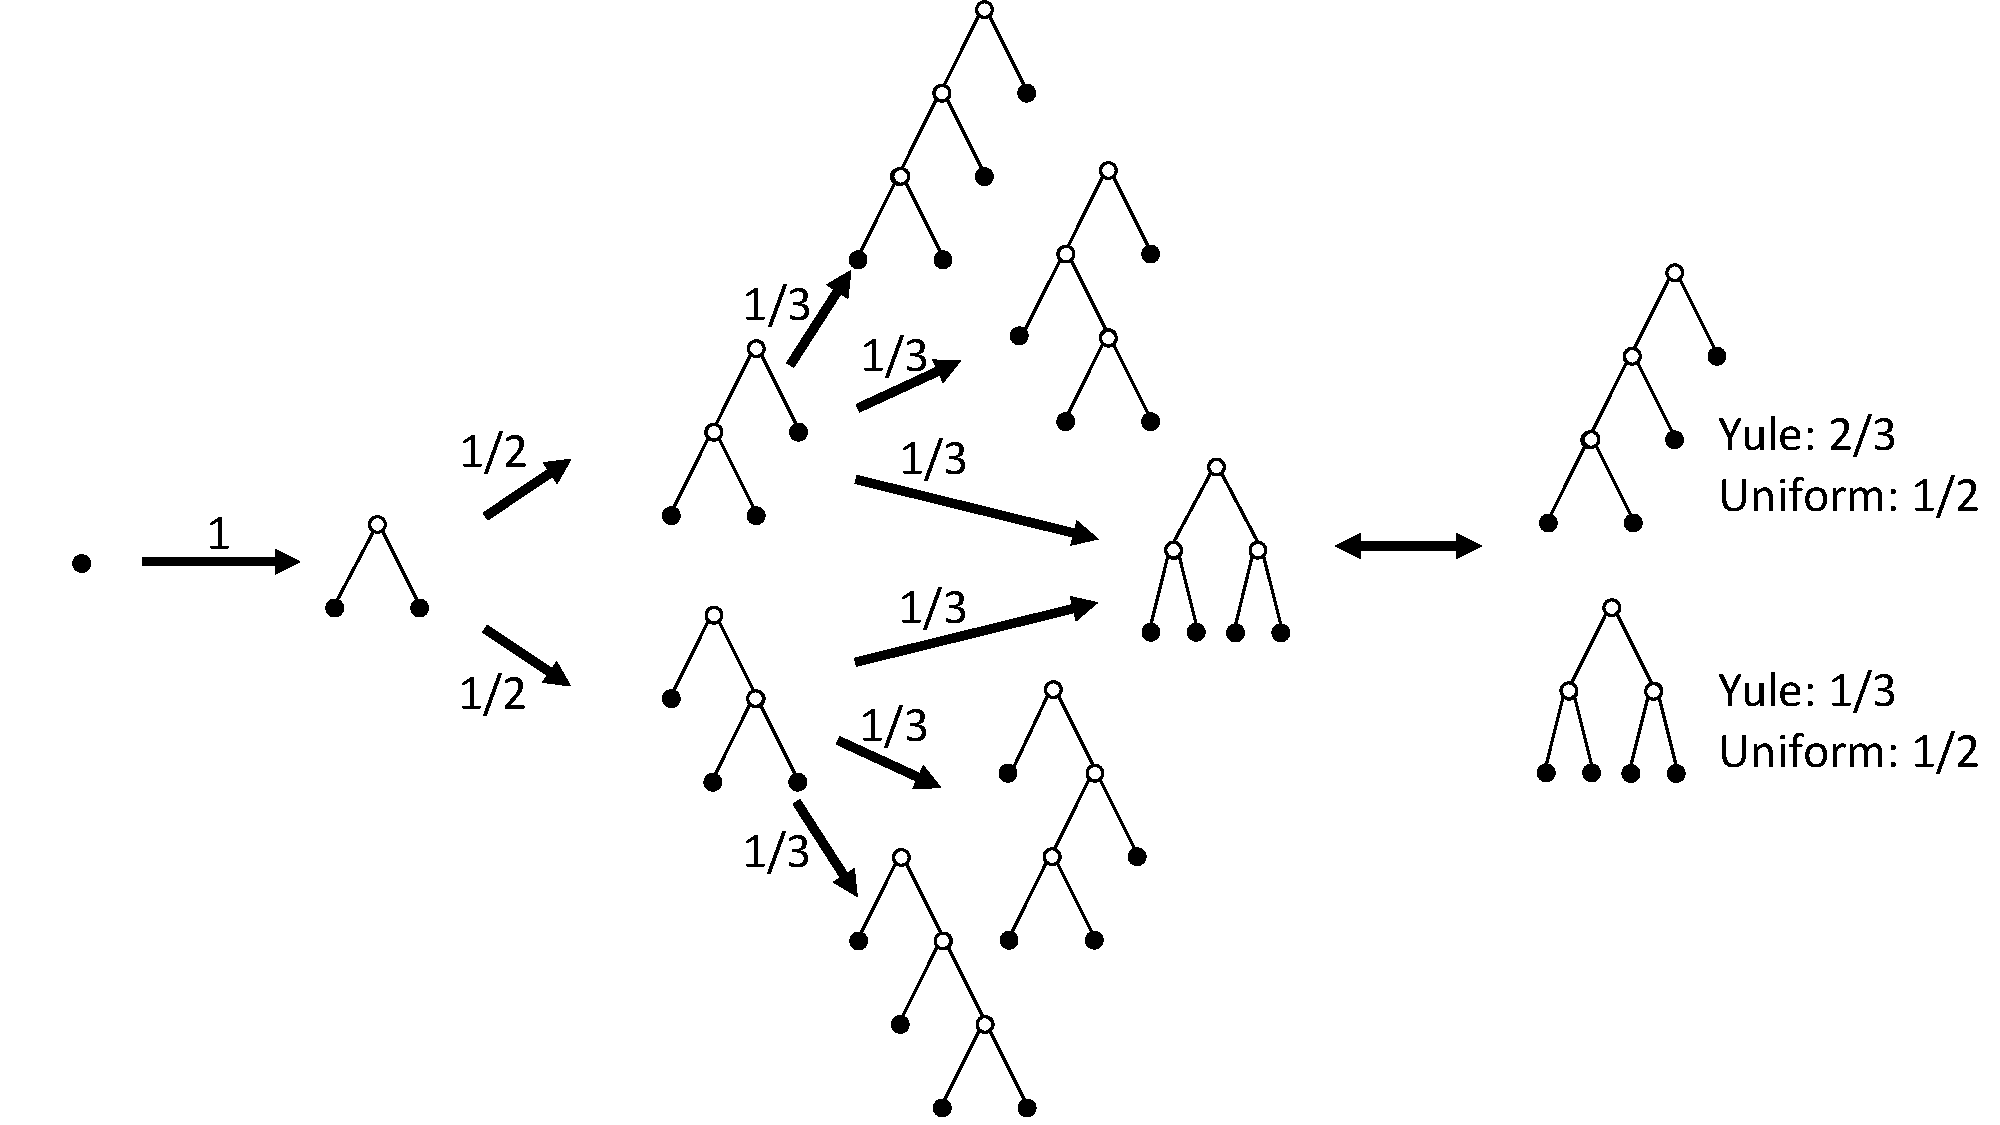
\includegraphics[width=\textwidth]{Chapter_trees/figures/yule-unif-figure.pdf}
    \caption{Comparison of probabilities for generation of trees on $4$ leaves under the Yule and uniform models.}
    \label{yule-unif-figure}
\end{figure}

The Yule and uniform models are statistical models which find their applications in evolutionary biology. Specifically, the Yule model, also known as the pure birth and coalescent model, is used when considering speciation rates and patterns \cite{aldous_stochastic_2001, steel_properties_2001}. The uniform model is typically encountered in evolutionary process considerations \cite{mooers_inferring_1997, steel_distributions_2000}. While simple, the two are are valuable null models for studying different aspects of evolution.


\section{Balancing binary trees according to $J^1$}
The balance index $J^1$ is defined on trees with arbitrary node out-degree distributions and node magnitudes \cite{lemant_robust_2021}. Depending on use case, this definition may be considered too broad. Specifically, in computer science the most commonly used tree is a binary tree.

\begin{definition}[Binary tree \cite{nievergelt_binary_nodate}]
	A \textbf{binary tree} is a rooted tree such that each node can have $0$, $1$, and $2$ children.
\end{definition}

While $J^1$ originally draws inspiration from the problem of quantifying properties of cancer phylogenetic trees \cite{noble_spatial_2022}, trees are encountered and used regularly in other fields, such as the broader realm of evolutionary biology, as well as computer science. However, one might notice that the notion of balance is used differently across those fields, being an effectively binary consideration in data structures, i.e. a tree can be balanced or unbalanced based on some measure \cite{nievergelt_binary_nodate}. In evolutionary biology, a finer scale is used, and comparisons between trees are more relevant \cite{mir_new_2013, mir_sound_2018, fischer_tree_2021}. Despite these differences, we have shown robustness of our method under common data gathering errors in biology \cite{lemant_robust_2021} and can further show that it generalises tree balance in data structures. Let us begin by defining the different measures of balance encountered in computer science literature.

\begin{definition}[Root balance score]
    The \textbf{root-balance score} $\rho(T_n)$ of a binary tree $T_n$ on $n > 1$ nodes is
    \begin{equation}\label{defrootbalscore}
        \rho(T_n) = \frac{l+1}{n+1},
    \end{equation}
    where $l$ is the number of nodes in the left subtree of $T_n$.
\end{definition}
Intuitively, one could imagine the root balance score as evaluating how well the tree could be balanced on a fulcrum placed under node $n$.

\begin{definition}[Weighted path length]
    Let $T$ be a rooted tree on $n$ nodes, and $\alpha_i$, $i=1,2,...$ the weights (or access frequencies) assigned to its nodes $v_i$. We define the \textbf{weighted path length} of tree $T$ as
    \begin{equation}\label{wpathdef}
        |T_n| = \sum_{v_i \in V(T)} \alpha_i \nu(v_i).
    \end{equation}
\end{definition}


\begin{remark}
    Let us rewrite the weighted path length in a more familiar way:
    \begin{equation*}
        |T| = \sum_{v_i \in V(T)} \alpha_i \nu(v_i) = \sum_{i \in V(T)} p_i \nu(i) = \sum_{i\in V(T)} S^*_i,
    \end{equation*}
    which is just the generalised Sackin index for tree $T$. 
\end{remark}
Consider then the following proposition.
\begin{proposition}[Lemant et al. \cite{lemant_robust_2021}]
    Let $T$ be a leafy tree on $n$ leaves with $d^+(i) = m > 1$. Then
    \begin{equation}
        J^1(T) = \frac{n\log_mn}{I_S(T)} \label{prop6}
    \end{equation}
    where $I_S$ is the Sackin index.
\end{proposition}
%state as a proposition and write down a brief proof properly - need to introduce proposition 6 before this happens also, could be a corollary
\begin{corollary}
    We can rewrite equation \eqref{prop6} for binary trees as 
    \begin{equation}
        J^1(T) = \frac{n\log_2n}{|\bar{T}|}. \label{corr6}
    \end{equation}
    This means that, for a fixed number of leaves $n$, minimising the weighted path length $|\bar T|$ is equivalent to maximising $J^1$. 
\end{corollary}

\begin{theorem}[Nievergelt and Wong \cite{wong_upper_1973}]
    Let $T_n$ be a binary node-tree with $n$ nodes and root balance score $\beta$. Then its total path length $|T_n|$ is bound from above by
    \begin{equation}\label{path_upper_bound}
        |T_n|_\text{upper} = (H(\beta))^{-1}(n+1)\log_2(n+1)-2n,
    \end{equation}
    where $H(\beta) = \beta\log_2\beta^{-1}+(1-\beta)\log_2(1-\beta)^{-1}$.
\end{theorem}

\begin{corollary}\label{j1_lower_bound_cor}
    There is a lower bound on $J^1$ for binary trees with $n$ nodes and root balance score $\beta$, and it equals
    \begin{equation}\label{j1_lower_bound}
        J^1_\text{lower} = \frac{n\log_2n}{|T_n|_\text{upper}}.
    \end{equation}
\end{corollary}

Corollary \ref{j1_lower_bound_cor} follows trivially from proposition \ref{j1_lower_bound} but represents a result which has a deeper connection to the fundamentals of information theory.

\begin{proposition}
    The Huffman method \cite{huffman_method_nodate} maximises $J^1$ on binary trees for a given set of node magnitudes.
\end{proposition}
\begin{proof}
    Consider a set of non-negative real numbers $F = \{\alpha_1, \dots, \alpha_m\}$. The Huffman method places larger numbers, i.e. nodes of higher magnitude, closer to the root, minimising the weighted path length as a result. By corollary \ref{j1_lower_bound_cor}, the Huffman method maximises $J^1$.
\end{proof}
As Huffman coding is an optimisation algorithm, we can use $J^1$ to measure how close a tree constructed using a given set of node magnitudes is to the maximally balanced binary tree on the same set. This means one can meaningfully measure how close an alternative algorithm which runs in a faster time complexity, such as arithmetic coding \cite{pasco_source}, gets to the optimal solution.

Let us now define the most common binary tree type one might encounter in computer science literature, binary search trees.
\begin{definition}[Binary search tree]
    A \textbf{binary search tree} $T_n$ over $n$ entries (w.l.g. numbers) $x_1,\dots,x_n$ is a labelled binary tree, each of whose nodes have been labelled with a distinct number chosen from $x1,\dots,x_n$ such that for each node $N$, all nodes in the left subtree of $N$ have a smaller $x_i$ as their label than $x_N$, and all nodes in the right subtree of $N$ have a larger number as their label than node $N$.
\end{definition}
The balance of binary search trees is usually measured by comparing the numbers of leaves in the left and right subtrees of the root. A more specific use case of binary search trees is for implementing dynamic data structures such as dictionaries \cite{tsakalidis_maintaining_1984}. For this purpose, weight-balanced trees are often used.
\begin{definition}[Weight-balanced tree]
    A weight-balanced tree is a binary search tree that stores the sizes of subtres in the nodes. That is, a node contains:
    \begin{itemize}
        \item key, of any type;
        \item value;
        \item left and right pointers to the child nodes;
        \item size.
    \end{itemize}
\end{definition}
\begin{definition}[Node balance]
    A node $i$, with children $i_l$ and $i_r$ and corresponding weights $w[i], w[i_l], w[i_r]$, is $\alpha$-weight-balanced if 
    \begin{align}
        w[i_l] \geq & \alpha w[i], \label{weight-balance-left} \\
        w[i_r] \geq & \alpha w[i], \label{weight-balance-right}
    \end{align}
    where $\alpha$ is a numerical parameter to be determined when implementing weight-balanced trees.
\end{definition}
Recall the general definition of $J^1$, where each internal node has an associated node balance. In the most general definition of $J^1$, equation \eqref{J1def}, the node balance $W_i$ of node $i$ can be any function $W_i: \mathbb{N}\to\mathbb{R}_{\geq 0}$ according to some property of node $i$ and its descendants. In other words, one may consider the node balance score $W_i$ as a generalisation of the root balance score since it calculates how evenly a node's descendants split the subtree rooted in it, as opposed to the overall tree structure. \par

The balance of weight-balanced trees is optimised dynamically through operations called rotations, which keep the weights of left and right subtrees within $\alpha$ of each other. Balance plays a major role in constructing good data structures in computer science, but computational efficiency is of much greater importance in the field, with balancing happening dynamically when new trees are initialised or nodes added to existing ones, other good examples being AVL trees and red/black trees \cite{noauthor_art_nodate}. The role of balance indices for static data structures is thus quite niche. However, by having a mathematically robust definition underpinning $J^1$, and considering general features of rooted trees, we have shown that it can easily be used far wider than just the original application of analysing cancer phylogenies. The connections between different tree use cases thus to show how one can construct powerful methods for general use without sacrificing specificity.

\begin{figure}
    \centering
    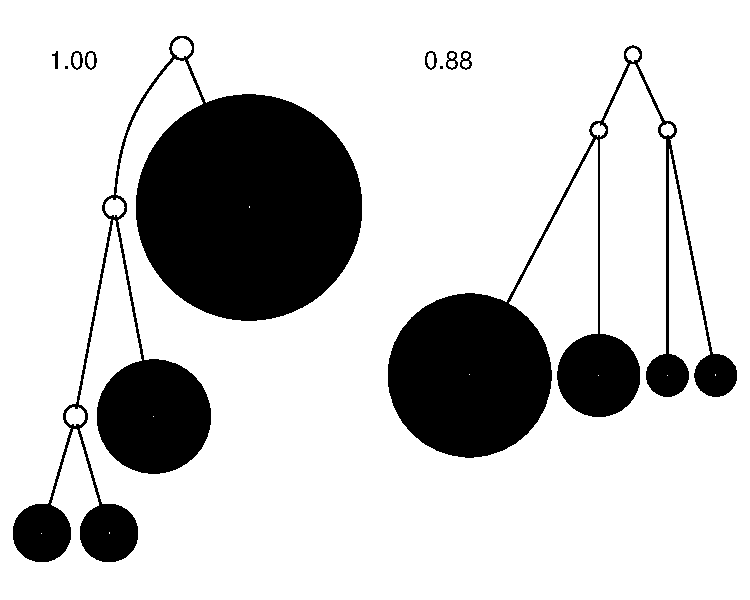
\includegraphics[width=0.8\textwidth]{Chapter_trees/figures/balcat.pdf}
    \caption{By including the node-balance function $W^1$ in $J^1$, we allow for the possibility of perfectly balanced caterpillars (left) and less balanced fully symmetric trees (right) based on the node size distribution in the tree.}
    \label{balcat}
\end{figure}

\iffalse
Since the index $J^1$ is related to Sackin's balance index and the Shannon entropy of a given leafy tree, as shown in our previous work \cite{lemant_robust_2021}, we can examine some further properties which results from this relationship. One of the first consequences of Proposition $6$ from the mentioned paper is that, for full $m$-ary cladograms, only the denominator of $J^1$ depends on the tree topology. That is
\begin{equation}
    J^1(T) = \frac{^1H(T)}{\sum_{i\in\mathcal{L}(T)}p_i\nu(i)\log m}, \label{prop6}
\end{equation}
where $\mathcal{L}(T)$ is the set of leaves of tree $T$, $^1H(T)$ is the tree's Shannon entropy, $m$ is the internal node degree, $\nu(i)$ is the node depth of leaf $i$, and $p_i$ is the weight of leaf $i$. This implies that, for a given set of node sizes and topology restricted to the set of bifurcating trees, $J^1$ is minimised using Huffman coding \cite{huffman_method_nodate}, i.e. clustering the heaviest nodes closest to the root, and letting the lightest ones populate the higher depth places (figure \ref{balcat}). While a straightforward result, it is an important demonstration of the universality of $J^1$. This implies that constructing an optimal search tree for a given set of frequencies will minimise $J^1$. Furthermore, consider the weighted path length of a weighted binary tree $T$, as defined in computer science literature \cite{nievergelt_binary_nodate}. One immediately sees that minimising the weighted path length is equivalent to maximising $J^1$ on leafy trees. These results enable us to compare the balance of completely different trees, as the behaviour of $J^1$ is consistent across the board. \\
If we consider a general weight-balance tree, the discussion is only slightly more complicated. In this context, a measure of balance one would commonly encounter in computer science literature is the weighted path length, calculated as 
\begin{equation}\label{weightedPL}
    |T| = \sum_{i\in V} \nu(i) p_i = \sum_{i\in\tilde{V}}S_i^*.
\end{equation}
The only difference between this metric and the Sackin index is the addition of weights in the more general case of trees with non-zero internal node sizes. This quantity is also the normalising factor of $J^1$ which implies a similar relationship between $J^1$ and $|T|$ to that of $J^1$ and Sackin's index, with the addition of the node balance score to account for even splits among a node's descendants. In fact, one might interpret the node balance score as a loose generalisation of the root balance score for each node,
\begin{equation}
    \rho(T_n) = \frac{l+1}{n+1},
\end{equation}
which is the ratio between the number of nodes in the subtree rooted in the left descendant of node $n$ and the number of nodes in the tree rooted in $n$. Furthermore, one could choose a node balance function based on the root balance but as shown in our previous paper, choosing $W^1$ related to the Shannon entropy gives $J^1$ certain desirable properties, a consequence of which is its relationship with Sackin's index. \par
\fi

        
\section{Expected value of $J^1$ under simple evolutionary processes}\label{expsection}
% proposition: E(J^1) approaches nlog_2n/E(I_S) as n goes to infinity under Yule and/or uniform and then prove, make it more like a mathematical paper with a sequence of propositions and proofs
% key things to add: looking at what happens to the upper bound, specifically in the uniform model case
% calculate limits for the edges of the Jensen gap as n goes to infty
For applications in evolutionary theory, an important property of balance indices is their expected value under an evolutionary process, as it tells us which process drove the tree into its current state. Equivalently to standard calculations in probability, one can obtain the expected value of a balance index by calculating the sum of the products of balance index values with the corresponding probability of the tree shape. 
\begin{definition}
Let process $P$ generate tree $T_i$ with probability $p(T_i)$ for $T_i\in\mathcal{T}_n$. The expected value of index $I_B$ on $n$ leaves under process $P$ is defined as
    \begin{equation}\label{expvaldef}
        \mathbb{E}_P^n(I_B) = \sum_{T_i\in\mathcal{T}_n} p(T_i)I_B(T_i).
    \end{equation}
\end{definition}

While the above definition seems quite general, in practice the generating process can introduce constraints on the set of trees. Two of the simplest, and most widely studied, processes of tree generation are the uniform model \cite{rosen_vicariant_1978} and the Yule model \cite{yule_iimathematical_1925}, which generate bifurcating trees. The expected value of a few indices, and even some higher moments in certain cases, are known for each of these tree generation processes \cite{mir_new_2013, m_coronado_sackins_2020, goh_two_2022}. Among these is the Sackin index, which is useful for our purposes. \par
Under the Yule model, the expected value of the Sackin index for trees on $n$ leaves is
\begin{equation}
    \mathbb{E}_Y^n(I_S) = 2n\sum_{i=2}^n \frac{1}{i},
\end{equation}
as shown in \cite{kirkpatrick_searching_1993}. Consider the relationship between $J^1$ and the Sackin index for bifurcating trees, which is directly derived from equation \eqref{prop6},
\begin{equation}\label{J1ISrel}
    J^1 = \frac{n\log_2 n}{I_S}.
\end{equation}
This means that the expected value of $J^1$ for a tree on $n$ leaves, generated under the Yule model is
\begin{equation*}
    \mathbb{E}_Y^n(J^1) = \mathbb{E}_Y^n(\frac{n\log_2 n}{I_S}) = n\log_2 n \mathbb{E}_Y^n(1/I_S).
\end{equation*}
We can rewrite this equation as
\begin{equation}
    \frac{1}{\mathbb{E}_Y^n(1/I_S)} = \frac{\mathbb{E}_Y^n(J^1)}{n\log_2n},
\end{equation}
which is the harmonic mean of the Sackin index. The harmonic mean under the Yule process is not a standard result in literature, nor have we been able to obtain a closed-form solution for this problem so far. We can, however, compare the harmonic and arithmetic means of $I_S$ by considering the Jensen gap
\begin{equation}\label{JensenGap}
    \mathcal{J}(f, X) = \mathbb{E}[f(X)] - f(\mathbb{E}[X]).
\end{equation}

\begin{theorem}[Liao and Berg \cite{liao_sharpening_2017}]\label{jensen_thm}
    Let $X$ be a one-dimensional random variable with mean $\mu$, and $P(X\in(a,b))=1$, where $\infty\leq a<b\leq \infty$. If $\phi(x)$ is a twice differentiable function on $(a,b)$, and
    \begin{equation*}
        h(x;\nu) = \frac{\phi(x)-\phi(\nu)}{(x-\nu)^2} - \frac{\phi'(\nu)}{x-\nu},
    \end{equation*}
    then
    \begin{equation}
        \inf_{x\in(a,b)}\{h(x;\mu)\}\mathrm{Var}(X) \leq \mathbb{E}[\phi(X)] - \phi(\mathbb{E}[X]) \leq \sup_{x\in(a,b)}\{ h(x;\mu) \}\mathrm{Var}(X).
    \end{equation}
\end{theorem}

\begin{proposition}\label{jensen_prop}
    Let $\mathbb{E}_Y(J^1)$ and $\mathbb{E}_U(J^1)$ be expectation values of $J^1$ under the Yule and uniform models respectively. Then:
    \begin{enumerate}[(i)]
        \item $\mathbb{E}_Y(J^1)\to\frac{n\log_2n}{\mathbb{E}_Y(I_S)}$,
        \item $\mathbb{E}_U(J^1)-\frac{n\log_2n}{\mathbb{E}_U(I_S)}$ is bounded from both sides,
    \end{enumerate}
    as $n\to\infty$.
\end{proposition}
\begin{proof}[Proof of proposition \ref{jensen_prop} (i)]
Let $\mu_Y$ be the expected value of the Sackin's index under the Yule process for trees on $n$ leaves, and $f(x)=\frac{1}{x}$. By theorem \ref{jensen_thm}
\begin{equation}\label{hxmuY}
    h(x;\mu_Y) = \frac{f(x)-f(\mu_Y)}{(x-\mu_Y)^2} - \frac{f'(\mu_Y)}{x-\mu_Y} = \frac{1}{x\mu_Y^2}.
\end{equation}
 We can then substitute this into the inequality given in the theorem
\begin{equation}\label{JensenApp}
    \frac{n\log_2n}{\frac{(n-1)(n+2)}{2}\mu_Y^2} \text{Var}_Y(I_S) \leq \mathbb{E}[J^1] - \frac{n\log_2n}{\mathbb{E}[I_S]} \leq \frac{n\log_2n}{\mu_Y^2n\log_2n}\text{Var}_Y(I_S),
\end{equation}
where the supremum and infimum of $h(x,\mu)$ are substituted with extremal values of the Sackin index on bifurcating trees \cite{fischer_extremal_2021}. The expectation of Sackin's index under the Yule model is a known quantity \cite{cardona_exact_2012}, and can be calculated as
\begin{equation}\label{yule_exp_sackin}
    \mathbb{E}_Y(I_S) = 2n\sum_{i=2}^n\frac{1}{i},
\end{equation}
as is its variance
\begin{equation}\label{varIS}
    \text{Var}_Y(I_S) = 7n^2 - 4n^2\sum_{i=1}^n\frac{1}{i^2} - 2n\sum_{i=1}^{n}\frac{1}{i} - n.
\end{equation}
Substituting these expressions into equation \eqref{JensenApp}, we find limits
\begin{align*}
    \frac{n\log_2n}{\frac{(n-1)(n+2)}{2}\mu_Y^2} \text{Var}_Y(I_S) &\stackrel{n\to\infty}{\sim} \frac{\log n\left(7n^2 - 4n^2\sum_{i=2}^n\frac{1}{i^2}-2n\sum_{i=2}^n\frac{1}{i}-n\right)}{4n^3\left(\sum_{i=2}^n\frac{1}{i}\right)^2} \\
    &\sim \frac{\log n}{n} \to 0
\end{align*}
for the lower bound on the gap, and
\begin{align*}
    \frac{n\log_2n}{\mu_Y^2n\log_2n}\text{Var}_Y(I_S) & = \frac{7n^2 - 4n^2\sum_{i=2}^n\frac{1}{i^2}-2n\sum_{i=2}^n\frac{1}{i}-n}{4n^2\left(\sum_{i=2}^n\frac{1}{i}\right)^2} \\
    & \stackrel{n\to\infty}{\sim} \frac{1}{\left(\sum_{i=2}^n\frac{1}{i}\right)^2} \to 0
\end{align*}
for the upper bound on the gap. The upper bound reaches a maximum at $n=13$ and is equal to approximately $0.0079$, while the lower bound reaches a maximum at $n=8$ and equals approximately $0.005$.
\end{proof}

% plot normalised Sackin vs J^1 for brooms, also colless vs J^1, check for cophenetic as well
% then have curves that *might* be tighter lower bounds of figure 7 in the original J^1 paper

\begin{figure}[h!]
    \centering
    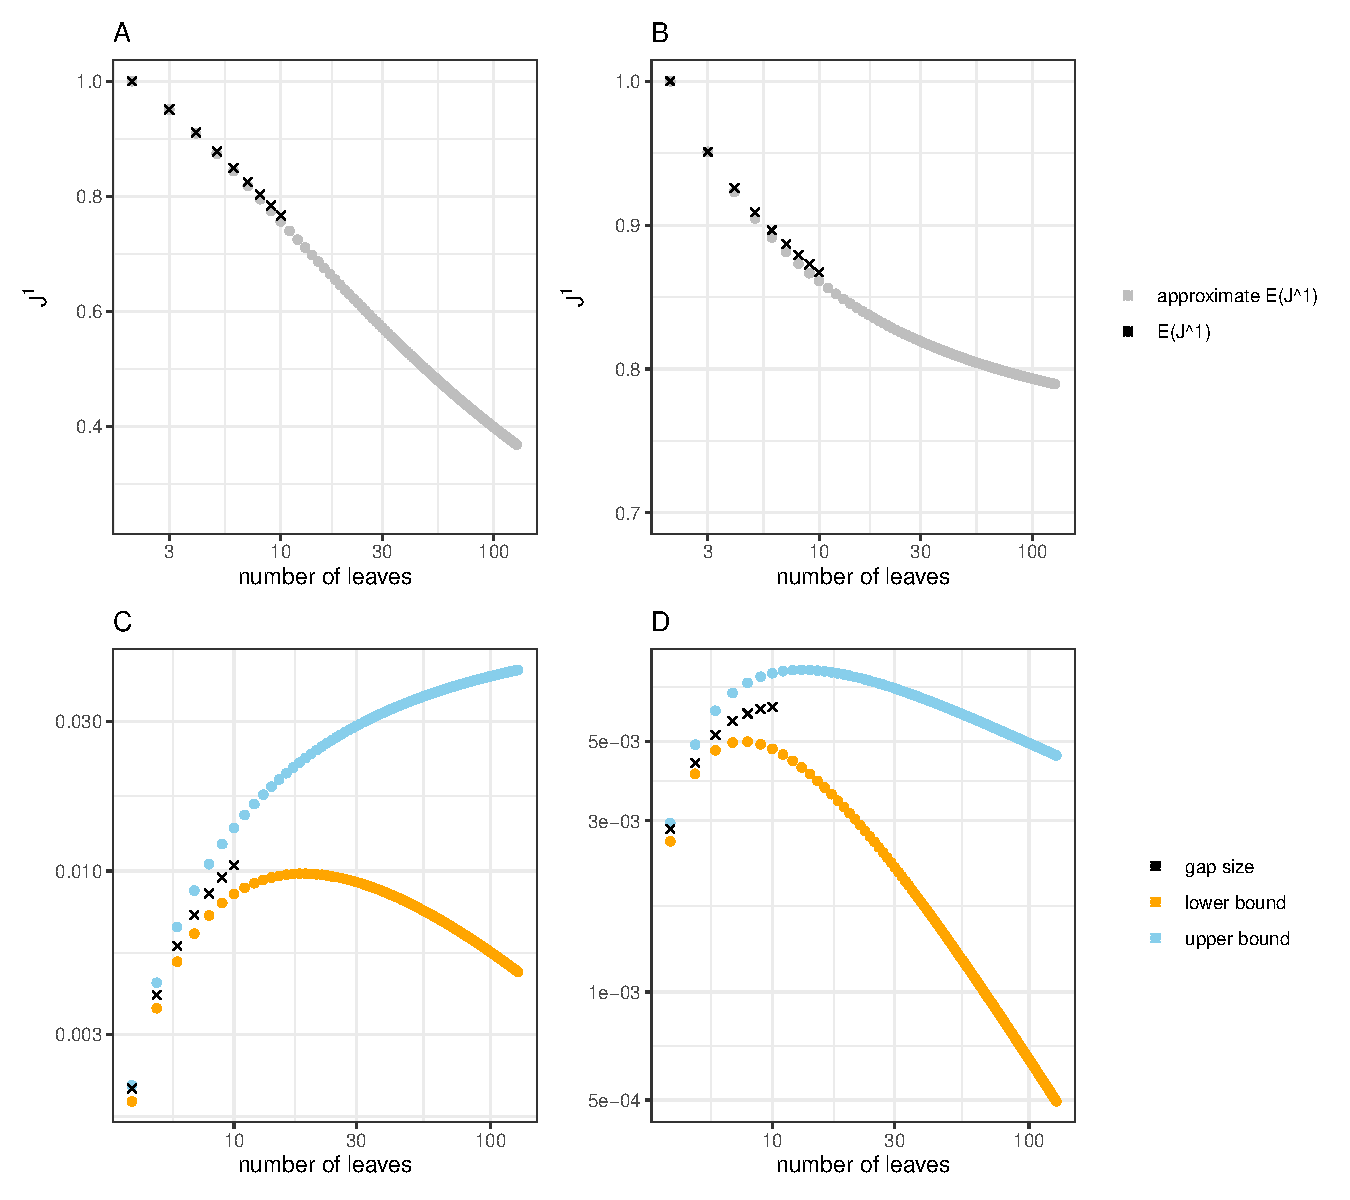
\includegraphics[width=\textwidth]{Chapter_trees/figures/jensenGapFigure.pdf}
    \caption{\textbf{Top row}: True values of $\mathbb E(J^1)$ for up to $10$ leaves were calculated manually, and the approximations up to $128$ leaves were calculated as $n\log_2n/\mathbb E(I_S)$. \textbf{A} --- uniform model, \textbf{B} --- Yule model.\\
    \textbf{Bottom row}: The Jensen gap of $\mathbb{E}(J^1)$ calculated for trees up to $128$ leaves under the uniform model (\textbf{C}), and the Yule model (\textbf{D}). The size of the gap is calculated as the difference between the true and approximate expected value, with the gaps for $2$ and $3$ leaves equal to zero as there is only one possible bifurcating tree shape for each of those values. Refer to tables \ref{table_yule} and \ref{table_unif} for numerical values of the gap size for the first several values of $n$.}
    \label{jensenfig} 
\end{figure}
In figure \ref{jensenfig}, we show behaviour of the Jensen gap and its bounds for $J^1$ under the Yule and uniform models.

Having a good approximation for the expected value of $J^1$ is a crucial result in the development of this index, as it allows us to employ it in the analysis of evolutionary processes on phylogenetic trees. The next step in this direction would be to obtain a closed-form solution for the expectation of $J^1$, as well as its variance.

\section{Analytic properties of the $J^1$ index}
A balance index is typically normalised by considering its extremal values for a given number of leaves \cite{fischer_tree_2021}. However, by its definition \cite{lemant_robust_2021}, $J^1$ follows a different normalisation procedure which in turn makes comparison of its values on trees of different sizes valid. The way $J^1$ was defined also makes it more complicated to define families of trees which maximise or minimise $J^1$ if we do not impose restrictions on the tree topology or node size distribution. In this section we do a bit of both, and consider only leafy trees with the out-degree of each internal node greater than $1$.

% look at the values of the edges of the relationship between the cophenetic index and J^1

	%\begin{itemize}
	%    \item a lot of this section is only relevant mathematically for completeness sake, rather than being applicable on real %data - especially the broom/caterpillar stuff
	%    \item \textbf{subsection} special trees - brooms, caterpillars, etc. present, discuss
	%    \item \textbf{subsection} tree ties - equivalence classes in index space, present, discuss
	%    \item \textbf{subsection} TBD
	%\end{itemize}
	
\subsection{Properties of $J^1$ on different tree families}
One may not encounter trees which yield extreme values of the balance index in practice often, if at all. However, it is still important to investigate the kinds of trees that maximise or minimise the index for the purposes of a complete mathematical discussion. 
	
\subsubsection{Some special tree topologies}
For most balance indices in use in evolutionary biology, the least balanced tree for a given number of leaves $n$ is the binary caterpillar tree. We have previously derived a general expression for leafy trees of this topology \cite{lemant_robust_2021}
\begin{equation}
    J^1(T_C) = \frac{2n\log_2n}{(n-1)(n+2)}.\label{caterpillar}
\end{equation}
Most balance indices in literature define the caterpillar topology as the least balanced one \cite{fischer_tree_2021}. Intuitively, this makes sense as balance is often associated with symmetry, and the caterpillar is the most asymmetric bifurcating tree. However, in the context of the $J^1$ index, tree topology is just one of a few factors which contribute to the balance score of a tree, especially since the index does not limit the space of trees to bifurcating ones. We also have to consider node sizes and, more specifically, how the population is split across different subtrees in the tree of interest. Let us consider a slightly altered caterpillar topology.
\par
\begin{figure}
    \centering
    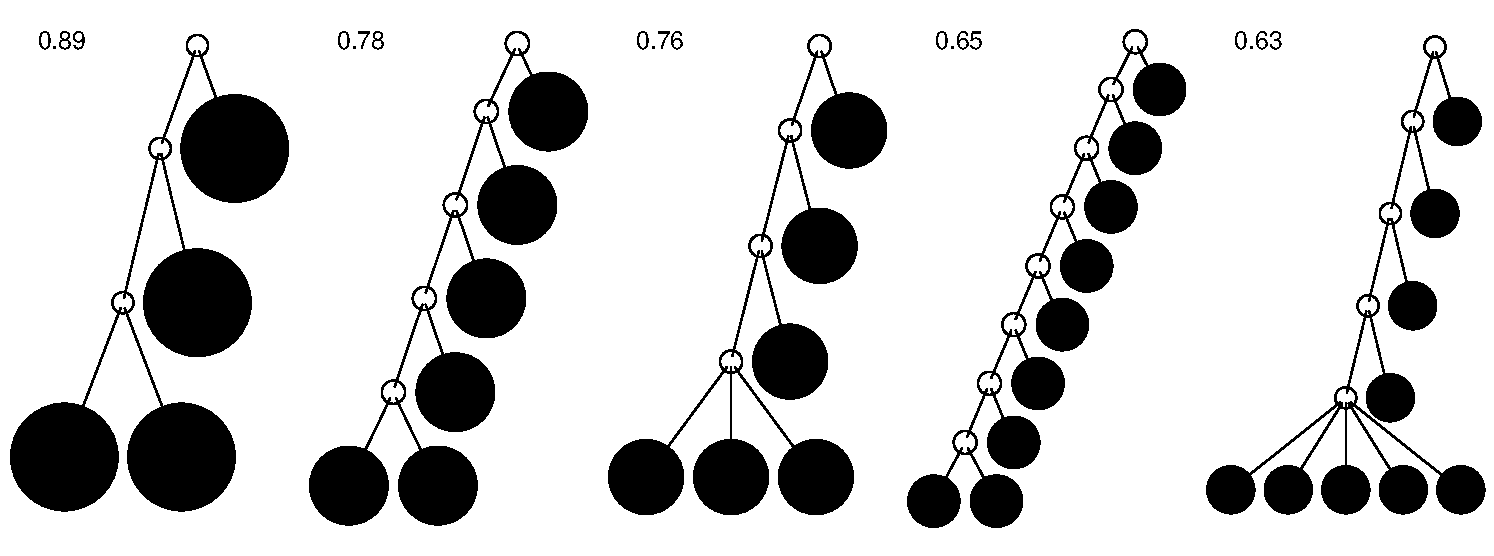
\includegraphics[width=\textwidth]{Chapter_trees/figures/example_figure_1.pdf}
    \caption{If we limit our search to leafy trees, the least balanced tree on a given number of leaves is not necessarily the caterpillar. Pictured are the caterpillar trees on $4$, $6$, and $9$ leaves, as well as minimally balanced brooms for $6$ and $9$ leaves, with corresponding $J^1$ values.}
    \label{example_figure_1}
\end{figure}

\begin{definition}
    Let $T_B$ be a leafy tree on $n$ leaves. Let every internal node of $T_B$ except for the one with the highest depth have out-degree $2$ such that one of its descendants is a leaf, and the other an internal node. Further, let the internal node most distant from the root have out-degree $k$. Then we call tree $T_B$ a \textbf{broom tree}.
\end{definition}

We can derive a general expression of $J^1$ for this family of trees.

\begin{proposition}\label{broom_prop}
    The value of $J^1$ for a broom tree $T_B$ on $n$ leaves, of which $k$ in the broom head is
    \begin{equation}
         J^1(T_B) = \frac{2}{(n+k)(n-k+1)}\left( n \log_2 n - k \log_2 k + k \right).\label{J1Tb}
    \end{equation}
\end{proposition}

We can also generalise the result of proposition \ref{broom_prop} slightly in the following way.

\begin{proposition}\label{q-broom-prop}
For a broom tree $T_{Bq}$ on $n$ leaves, of which $k$ in the broom head, such that the sizes of leaves in the head sum to $q$, $q\in \mathbb R$, and the leaves in the ``handle" all of equal size $1$, the value of $J^1$ is
    \begin{align*}
        J^1(T_{Bq}) = &\frac{1}{(n-k+1)(q+(n-k)/2)}\\
        &\times\left( q\log_k q-\sum_{i=1}^{k}l_i\log_k l_i+(q+n-k)\log_2(q+n-k) - q\log_2q \right),\numberthis\label{J1Tbq}
    \end{align*}
        where $l_1,\dots,l_k$ are the leaf sizes which add up to $q$.
\end{proposition}

In figure \ref{example_figure_1} we show that the caterpillar is not the minimally balanced leafy tree for a few tree sizes. To take it a step further, consider the following proposition. 

\begin{proposition}\label{cat_prop}
    For leafy trees on $n$ leaves and no linear parts, the caterpillar minimises $J^1$ iff $n<5$.
\end{proposition}
\begin{proof}
    Let $J^1_B(n,k)$ denote the value of $J^1$ on a broom tree with $n$ leaves, of which $k$ in the broom head. Then
    \begin{align}
        J^1_B(n,2) = & \frac{2n\log_2n}{(n+2)(n-1)}, \label{j1bn2}\\
        J^1_B(n,3) = & \frac{2}{(n+3)(n-2)}(n\log_2n - 3\log_2 3 + 3).\label{j1bn3}
    \end{align}
    Consider the case when $J^1_B(n,2) < J^1_B(n,3)$. Plugging in equations \eqref{j1bn2} and \eqref{j1bn3}, we can rearrange the inequality to find
    \begin{equation}
        8n\log_2n - 6(n^2+n-2)\log_2 3 + 6(n^2+n-2) > 0,
    \end{equation}
    which changes sign at $0, 0.667, 1$ and $4.168$. Setting the first derivative of this expression to zero 
    \begin{equation*}
        8\log_2n+\frac{8}{\log 2}-(12n+6)\log_2 3 + 12n + 6 = 0
    \end{equation*}
    we find solutions around $n=0.822$ and $n=2.888$, the latter of which signifies a local maximum. Therefore, as $n$ can only take positive integer values, valid solutions for which the caterpillar is less balanced than the broom with $3$ leaves in the broom head according to the index $J^1$ are $3$ and $4$, with the $k=3$ broom being less balanced otherwise.
\end{proof}

This proposition gives us a threshold for the number of leaves at which the caterpillar is not longer the minimally balanced tree for the given number of leaves, which sets $J^1$ apart from traditionally defined balance indices. This comes with the benefit of the new index's robustness to removal of small nodes, universality, and generality. However, we are yet to prove the following statement.

\begin{conjecture}\label{conj}
    For leafy trees on $n$ leaves and no linear parts, the tree that minimises $J^1$ belongs to the broom family.
\end{conjecture}

\subsubsection{Behaviour as $n\to\infty$}
    
    \begin{figure}[h!]
        \begin{center}
        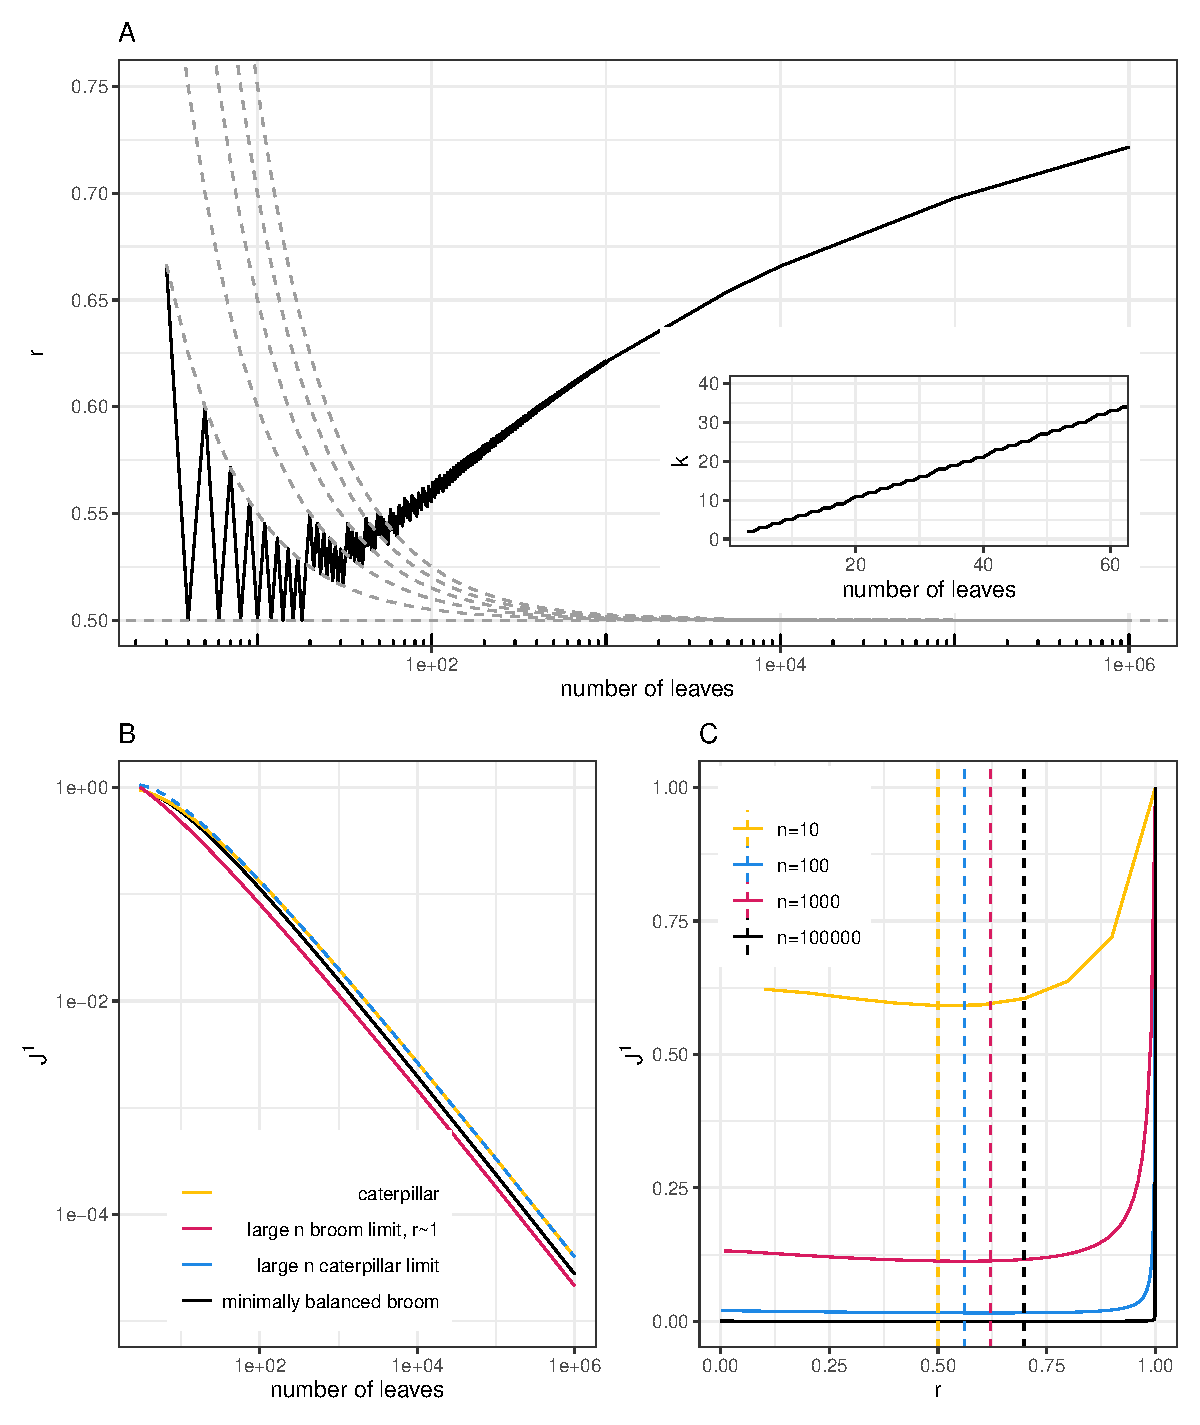
\includegraphics[width = \textwidth]{Chapter_trees/figures/figures_updated.pdf}
        \caption{The labels used in the figures are as above - $n$ for number of leaves, $k$ for number of leaves in the broom head, $r=n/k$. \textbf{A:} Value of $r$ for which the minimum value of $J^1$ is obtained on leafy trees. Trees on $n$ leaves which satisfy $r = \frac{n+a}{2n}$, for $a=0,1,2,\dots$ lie on the dashed grey lines. \textbf{B:} Behaviour of caterpillar and broom for different values of $n$. \textbf{C:} $J^1$ for different broom trees on a given number of leaves using equation \eqref{J1Tb}. The dashed lines indicate the value of $r$ for which $J^1$ is minimal.}
        \label{Rfigures}
        \end{center}
    \end{figure}

    % try and figure out a closed form expression for the bounds on n vs r - could help figure out what's going on in the formula
    %add m-ary caterpillar curves to the figure as well - relevant
We have derived general behaviour of $J^1$ on broom and caterpillar trees for a given number of leaves $n$. However, as some of the equations implied are not analytically solvable (e.g., conjecture \ref{conj}) we also explore asymptotic behaviour of $J^1$.
%find general expression for full m-ary caterpillar
%simplest case caterpillar is for bifurcating trees, now we extend to full m-ary trees
If we let $n\to\infty$, the value of $J^1$ for the caterpillar from equation \eqref{caterpillar} will behave like
    \begin{equation}
        \lim_{n\to\infty} J^1(T_C) = \frac{2\log_2n}{n}. \label{caterpillarlim}
\end{equation}

As $J^1$ is not limited to trees with equal leaf sizes, there is a threshold we can impose on the broom tree beyond which the caterpillar is less balanced.

\begin{proposition}\label{p-broom-prop}
    Let $T_B(n)$ be a broom tree on $n$ leaves such that the leaves on the handle and head have sizes $f$ and $fp$ respectively, and $T_C(n)$ be a caterpillar tree on $n$ leaves of equal sizes $f$. Then
    \begin{equation}\label{p-broom-cond}
        J^1(T_B) > J^1(T_C) \text{\quad iff \quad} p<\frac{1}{2},
    \end{equation}
    as $n\to\infty$.
\end{proposition}

For broom trees, the behaviour is a little more complicated and, perhaps, counterintuitive. Consider the following.
\begin{proposition}\label{ropt_prop}
    Let $\mathcal{T}_B(n)$ be the set of all broom trees on $n$ leaves, $r = \frac{k}{n}$ where $k$ is the number of leaves in the broom head for a given tree, and $r_\text{opt}$ the value of $r$ which minimises $J^1$ for a given $n$. Then $r_\text{opt}\to 1$ as $n\to\infty$.
\end{proposition}
The proposition says that most leaves on a minimally balanced broom tree will be concentrated in the head, with comparatively few on the handle, resembling a start tree more closely than a caterpillar tree. However, one must take into account how imbalanced the nodes above the broom head are, since one of their subtrees contains most of the tree's leaves, whereas the other is a single leaf. 

\par 

Finding the true value of $k$ which minimises $J^1(T_B)$ analytically is difficult. The derivative with respect to $k$ of equation \eqref{J1Tb} yields a transcendental equation which is not analytically solvable.
    
\section{Discussion}
        %\begin{itemize}
         %   \item $J^1$ is not a traditional balance index, contains more information, more widely applicable
	%	\item while more general/universal than other indices, $J^1$ does not account for all information one might wish to include in a tree --- branch length discussion?
	%\end{itemize}

The main aim of this paper was to explore deeper analytic properties of the robust, universal balance index $J^1$ and start finding its place in the broader context of tree balance by extending past results and uncovering new connections. \par
There are still areas where the index $J^1$ falls short in terms of generality. The balance of a tree whose branch lengths differ is not a case that the new index can handle. This opens up the possibility of further generalisation of the index and future research.\par
Finally, we only touched upon directly obtainable relationships without considering different real-world use cases of the index and the implications of equation \eqref{prop6}. This is another avenue of future research as there may exist a relationship between the way indices vary with time and the underlying evolutionary process growing the associated tree.

